%% LyX 2.4.2.1 created this file.  For more info, see https://www.lyx.org/.
%% Do not edit unless you really know what you are doing.
\documentclass[12pt,english]{beamer}
\usepackage{mathpazo}
\renewcommand{\familydefault}{\rmdefault}
\usepackage[T1]{fontenc}
% \usepackage[latin9]{inputenc}
\setcounter{secnumdepth}{3}
\setcounter{tocdepth}{3}
\usepackage[active]{srcltx}
\usepackage{amsthm}
\usepackage{amssymb}
\usepackage{tikz}
\usepackage[authoryear]{natbib}

\setbeamertemplate{navigation symbols}{}

\makeatletter
%%%%%%%%%%%%%%%%%%%%%%%%%%%%%% Textclass specific LaTeX commands.
% this default might be overridden by plain title style
\newcommand\makebeamertitle{\frame{\maketitle}}%
% (ERT) argument for the TOC
\AtBeginDocument{%
  \let\origtableofcontents=\tableofcontents
  \def\tableofcontents{\@ifnextchar[{\origtableofcontents}{\gobbletableofcontents}}
  \def\gobbletableofcontents#1{\origtableofcontents}
}
\theoremstyle{definition}
\newtheorem*{example*}{\protect\examplename}
\theoremstyle{definition}
\newtheorem*{defn*}{\protect\definitionname}
\theoremstyle{plain}
\newtheorem*{thm*}{\protect\theoremname}
\newtheorem*{assumption*}{\protect\assumptionname}

%%%%%%%%%%%%%%%%%%%%%%%%%%%%%% User specified LaTeX commands.
\AtBeginDocument{%
   \let\origtableofcontents=\tableofcontents
   \def\tableofcontents{\@ifnextchar[{\origtableofcontents}{\gobbletableofcontents}}
   \def\gobbletableofcontents#1{\origtableofcontents}
 }\usepackage[english]{babel}
\usepackage{babel}

%\usetheme{Boadilla}
\usetheme{Madrid}
% \usecolortheme{orchid}
\usecolortheme{spruce}
% \usecolortheme{beaver}

\providecommand{\assumptionname}{Assumption}

\setbeamercovered{transparent}

\usepackage{colortbl}

\usefonttheme[onlymath]{serif}
%%%%%%%%%%%%%%%%%%%%%%%%

% For tables
\usepackage{multirow}
\usepackage{array}
\usepackage{rotating}
\usepackage{longtable}
\usepackage{float}
\usepackage{booktabs}


% For figures
\usepackage{caption}
\usepackage{subcaption}

\makeatother

\usepackage{babel}
\providecommand{\definitionname}{Definition}
\providecommand{\examplename}{Example}
\providecommand{\theoremname}{Theorem}

\title[panel]{Panel Data}
\author[]{Zhentao Shi}
\date[]{The Chinese University of Hong Kong}

\begin{document}

\frame{\titlepage}

% Uncomment if you want a table of contents slide
% \begin{frame}
%     \tableofcontents
% \end{frame}


\begin{frame}{Data}

\begin{center}
    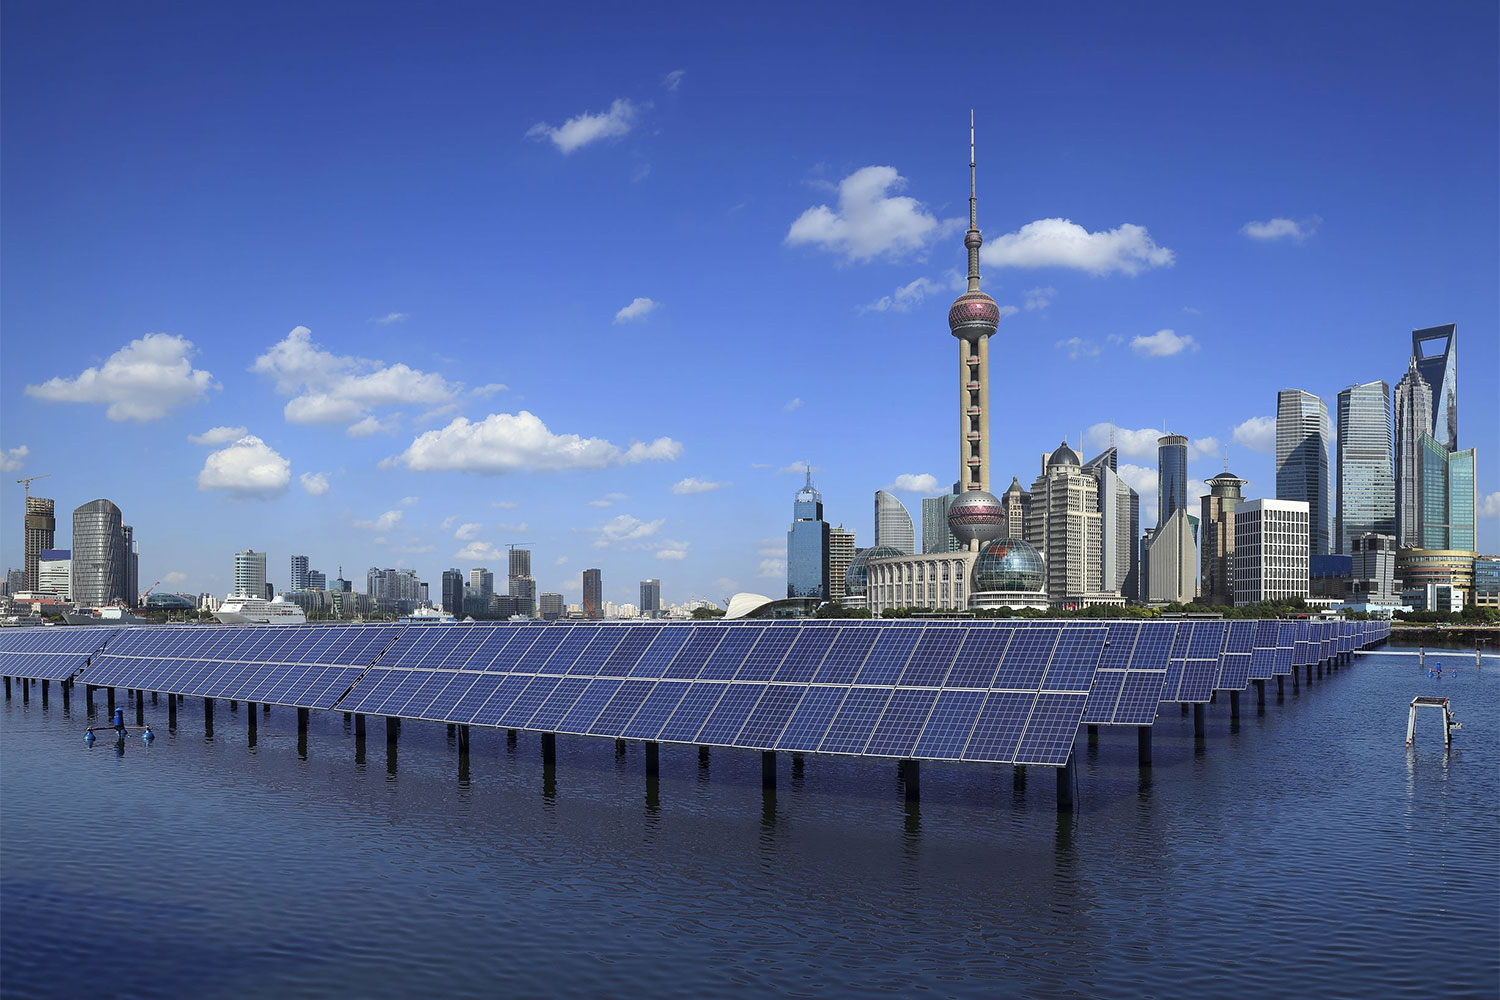
\includegraphics[width = 0.5 \textwidth]{fig/solar-panels.jpg}
\end{center}

    \begin{itemize}
        \item Cross-sectional datasets collected at different time points  
        \item Group-specific intercept  (one way to handle endogeneity)
        \item Real data: \url{https://www.kaggle.com/code/frankshi0/penn-world-table}
    \end{itemize}
\end{frame}



\begin{frame}[plain]{Panel Data Structure}
    \begin{itemize}
        \item The same individuals are observed over time $t=1,\ldots,T$  
        \item Independent across $i=1,\ldots,N$  
    \end{itemize}

\begin{center}
        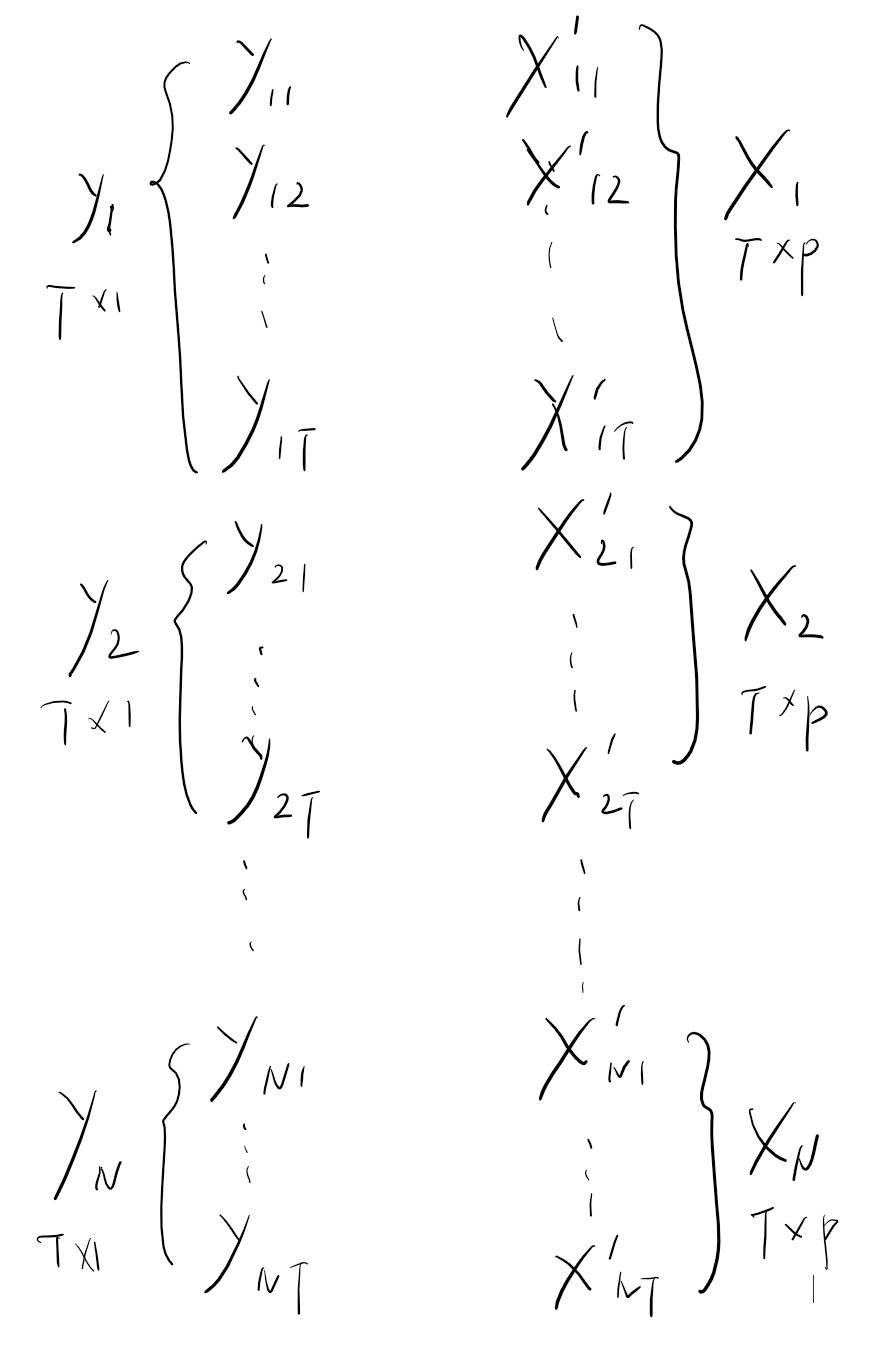
\includegraphics[width=0.30\linewidth]{fig/panel_data_yx.png}
\end{center}

Real data: \url{https://www.kaggle.com/datasets/frankshi0/nber-ces-manufacturing-industry-database/code}

\end{frame}





\begin{frame}{Panel Data Regression}
    \begin{itemize}
    
        \item Temporal dependence is allowed within a \textbf{group} over $t=1,\ldots,T$ for the same $i$.  
            \begin{equation*}
                y_{it}=c +X_{it}'\beta +\varepsilon_{it} 
            \end{equation*}  
            with $E(\varepsilon_{it} ) = 0$.
        \item $\varepsilon_{it}$ may be correlated with $X_it$.
        \item \textbf{Composite error}: 
        $$\varepsilon_{it}=\alpha^*_{i} + u_{it}$$         with $\mathrm{cov} (u_{it}, X_{it}) = 0$
    \end{itemize}
\end{frame}


\section{Fixed Effect Models}
\frame{\sectionpage}


\begin{frame}{Fixed Effects}
    \begin{itemize}
        \item Consistency of OLS counts on 
        $\mathrm{cov}(\varepsilon_{it}, X_{it}) = \mathrm{cov}(\alpha^*_{i}, X_{it}) + \mathrm{cov}(u_{it},X_{it})=0$.
        
        \item Example
        \begin{itemize}
            \item Production function (Mundlak, 1961)
 $$y_{it}= c +X_{it}'\beta + m_i \gamma + u_{it} $$
 where $m_i$ is the ``management quality'' of a firm (usually unobservable).
        \item $m_i\gamma$, which can be correlated with $X_{it}$, is captured by $\alpha^*_i$
        \end{itemize}
        
        \item  $\alpha^*_{i}$ can be potentially endogenous (correlated with $X_{it}$)
    
    \end{itemize}
\end{frame}




\begin{frame}{Static Linear Model}
    \begin{itemize}
        \item Model 
        \begin{align*}
          y_{it} & =c +X_{it}'\beta +\varepsilon_{it}  \\  
                 & =(c + \alpha^*_i) +X_{it}'\beta + u_{it}  \\
                 & = \alpha_{i} +X_{it}'\beta + u_{it}  
        \end{align*}
    where $ \alpha_{i} = c + \alpha^*_i$ is the new \textbf{individual-specific}
    intercept. Also called the \textbf{fixed effect}.
    \item $\beta$ is a $p$-dimensional \textbf{homogenous} slope coefficient 

\bigskip

    \item $(N+p)$ Parameters $(\alpha_{1 },\alpha_{2 }, \ldots, \alpha_{N }; \beta) $
        
    \end{itemize}
\end{frame}



\begin{frame}{Least Squares Dummy Variable Estimator}
    \begin{itemize}
        \item Direct Estimation 
        $$y_{it} = \sum_{j=1}^N \alpha_{j} \mathbf{I}(i=j) +X_{it}'\beta +u_{it}  $$
    \end{itemize}

\begin{center}
        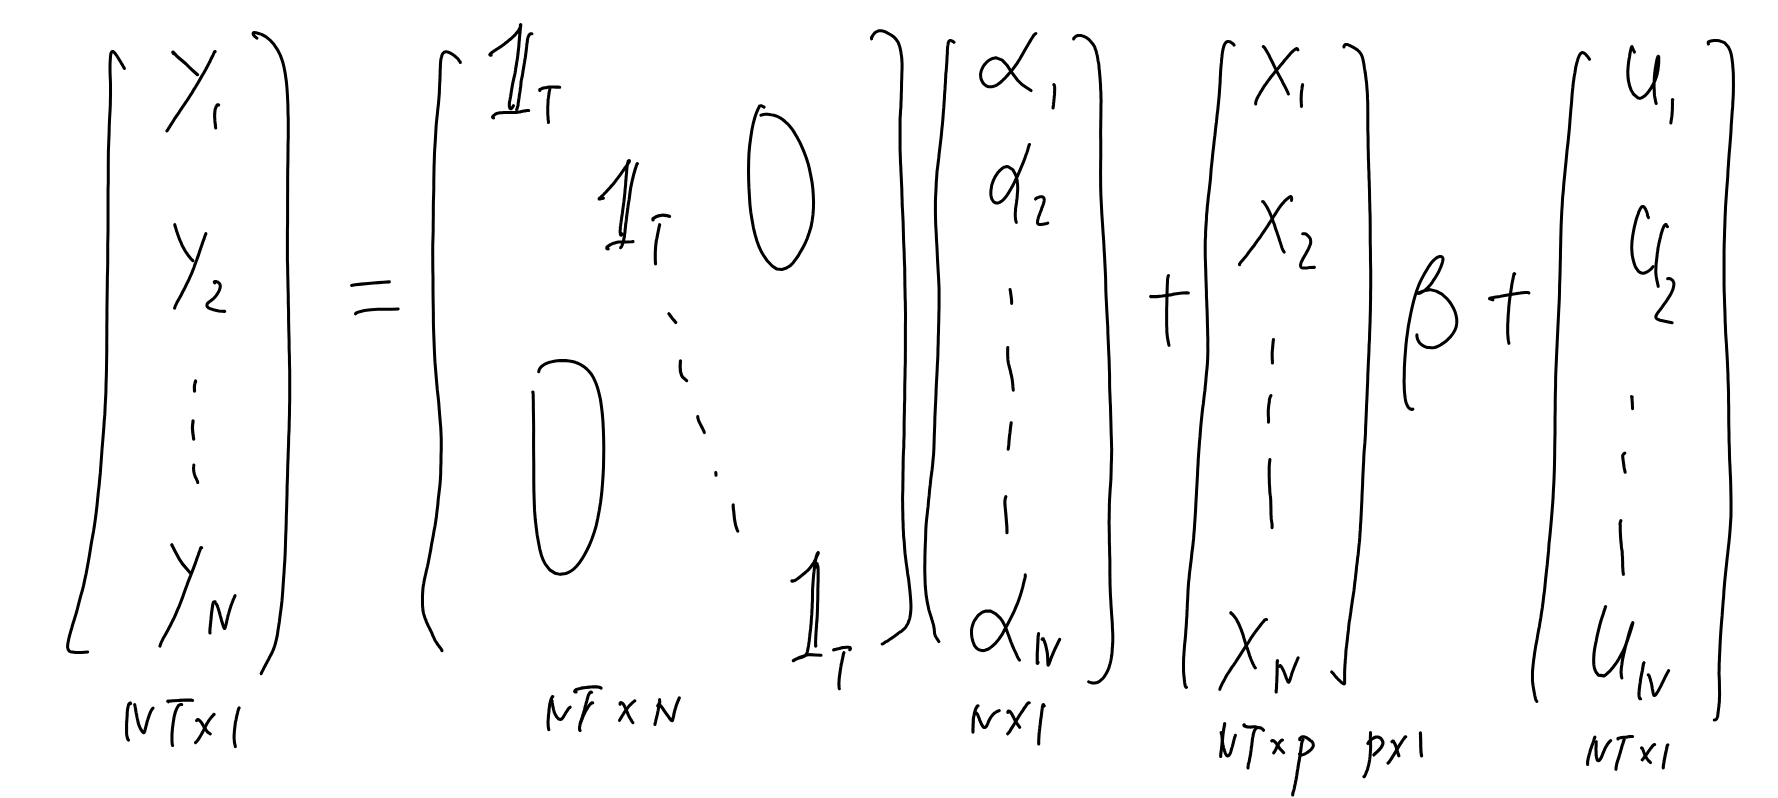
\includegraphics[width=0.8\linewidth]{fig/panel_data_reg.png}
\end{center}
    
\end{frame}



\begin{frame}{Within-Group Transformation}
    \begin{itemize}
        \item Inner-outer optimization: given any $\beta$, the OLS estimator
        $$\hat{\alpha}_{i} = T^{-1} \sum_{t=1}^T (y_{it} - X'_{it} \beta)
          = \bar{y}_{i} - \bar{X}'_{i} \beta, $$
          where $\bar{y}_i = T^{-1} \sum_{t=1}^T y_{it}$ is the \textbf{within group average}, and so is $\bar{X}_i$.
        \item Substitute $\hat{\alpha}_{i}$ into $y_{it} = \alpha_{i} +X_{it}'\beta + u_{it}$ and rearrange:
        $$\tilde{y}_{it}=\tilde{X}'_{it}\beta +\tilde{u}_{it}$$
         where $\tilde{y}_{it}=y_{it}-\overline{y}_{i}$ is the \textbf{within-group transformation}, and  $\tilde{X}_{it}$ and $\tilde{u}_{it}$ are defined similarly.
         
        \item This transformation eliminates the $N$ parameters $(\alpha_{i})_{i=1}^N$.
    \end{itemize}
\end{frame}








\begin{frame}{Alternative Interpretation of Within-Group Transformation}
    \begin{itemize}
        
        \item Recall the model $$y_{it} = \alpha_i + X_{it}^{\prime}\beta + u_{it}.$$
        \item For each $i$, average over $t = 1, \ldots, T$:
        \[
        \bar{y}_i = \alpha_i + \bar{X}_i^{\prime}\beta + \bar{u}_i.
        \]
        \item Subtraction:
        \[
        \tilde{y}_{it} = \tilde{X}_{it}^{\prime}\beta + \tilde{u}_{it}.
        \]
         eliminates the fixed effects.
        \item No intercept, by construction.
    \end{itemize}
\end{frame}


\begin{frame}{ Data in Blocks}

\begin{itemize}
    \item Stack into long vector/matrix of all data
    
    \[
    \underset{NT \times 1}{
    \begin{bmatrix}
        \tilde{y}_1 \\
        \tilde{y}_2 \\
        \vdots \\
        \tilde{y}_N
    \end{bmatrix}}
    =
    \underset{NT \times p}{
    \begin{bmatrix}
        \tilde{X}_1 \\
        \tilde{X}_2 \\
        \vdots \\
        \tilde{X}_N
    \end{bmatrix}}
    \underset{p \times 1}{\beta}
    +
    \underset{NT \times 1}{
    \begin{bmatrix}
        \tilde{u}_1 \\
        \tilde{u}_2 \\
        \vdots \\
        \tilde{u}_N
    \end{bmatrix}}.
    \]
\item Compact expression of data:
    \[
    \tilde{Y} = \tilde{X}\beta + \tilde{u}.
    \]
\end{itemize}

\end{frame}





\begin{frame}{Within Estimator}
    \begin{itemize}
        \item Within estimator (or equivalently the FE estimator):
        \[
            \widehat{\beta} _{FE}=\left(\tilde{X}'\tilde{X}\right)^{-1}\tilde{X}'\tilde{Y}  
        \]

        \item The fixed effects are estimated as
        $$\hat{\alpha}_{i} =  \bar{y}_{i} - \bar{X}'_{i} \hat {\beta}_{FE} $$
        
        \item Consistency is achieved if strict exogeneity holds.
    \end{itemize} 
    % \begin{assumption*}[FE.1]
        % $E\left[u_{it}|\alpha_{i},\mathbf{X}_{i}\right]=0$ where $\mathbf{X}_{i}=\left(X_{i1},\ldots,X_{iT}\right)$. 
    %\end{assumption*} 
    %\begin{assumption*}[FE.2]
     % $\mathrm{var}\left(u_{i}|\alpha_{i},\mathbf{X}_{i}\right)=\sigma_{u}^{2}I_{T}$. 
    %\end{assumption*}
\end{frame}




\begin{frame}{Strict Exogeneity}
    \begin{itemize}
        \item A necessary condition for the consistency of $\widehat{\beta}_{FE}$:
        \[
        E\left[ \left(X_{it} - \bar{X}_i\right)\left(u_{it} - \bar{u}_i\right) \right] = 0.
        \]

        \item A sufficient condition is \textbf{strict exogeneity}:
        \[
        E\left[ X_{it} u_{is} \right] = 0 \quad \text{for all } s, t \in \{1, \ldots, T\}.
        \]

        \item Interpretation: no correlation of the error term $u_{is}$ with the regressor $X_{it}$ in the past, present, and future.
    \end{itemize}
\end{frame}


\begin{frame}{ Exogeneity}
    \begin{itemize}
        \item Notice that 
        \[
        \tilde{X}_{it} = X_{it} - \frac{1}{T} \sum_{t=1}^T X_{it}
        = \left(1 - \frac{1}{T}\right) X_{it} - \frac{1}{T} \sum_{s \neq t} X_{is},
        \]
        is a linear combination of \(\{X_{i1}, \ldots, X_{iT}\}\).

        \item \textbf{Contemporaneous exogeneity}:
        $E\left(X_{it} u_{it}\right) = 0 \quad \text{for all } t \in \{1, \ldots, T\}.$

        \item \textbf{Sequential exogeneity}:
        $E\left(u_{it} X_{is} \right) = 0 \quad \text{for all } s \leq t \in \{1, \ldots, T\}.$ The error term is uncorrelated with the last and present regressor.

        \item Neither of the above two kinds of exogeneity produces consistent \(\widehat{\beta}_{FE}\).
    \end{itemize}
\end{frame}





\begin{frame}{Variance Estimation for FE}
    \begin{itemize}
        \item Under homoskedasticity:
        \[
            \widehat{\sigma}_{u}^{2}=\frac{1}{n\left(T-1\right)}\sum_{i=1}^{n}\sum_{t=1}^{T}\widehat{\tilde{u}}_{it}^{2}.
        \]
        where $\widehat{\tilde{u}}=\tilde{y}_{it}-\tilde{X}_{it}\widehat{\beta} _{FE}$  
        
        \item Asymptotic normality
        \[            \left(\widehat{\sigma}_{u}^{2}\left(\tilde{X}'\tilde{X}\right)^{-1}\right)^{-1/2}\left(\widehat{\beta} _{FE}-\beta ^{0}\right)\Rightarrow N\left(0,I_{K}\right).
        \]
        
    \end{itemize}
    % \begin{theorem}[FE Asymptotic Normality]
      
        
    % \end{theorem}
\end{frame}



\begin{frame}{First Difference (FD)}
    \begin{itemize}
    \item Alternative way to eliminate FE
        \item Recall 
        \[
        y_{it} = \alpha_i + X_{it}^{\prime}\beta + u_{it},
        \]
        \[
        y_{i,t-1} = \alpha_i + X_{i,t-1}^{\prime}\beta + u_{i,t-1}.
        \]

        \item Subtraction:
        \[
        \Delta y_{it} = \Delta X_{it}^{\prime}\beta + \Delta u_{it},
        \]
        where \(\Delta y_{it} = y_{it} - y_{i,t-1}\) is the first-differenced variable, and \(\Delta X_{it}\) and \(\Delta u_{it}\) are defined similarly.

        \item Collect the FD variables into \(\Delta Y\) and \(\Delta X\):
        \[
        \Delta Y \quad \text{is of size } N(T-1) \times 1,
        \]
        \[
        \Delta X \quad \text{is of size } N(T-1) \times p.
        \]
    \end{itemize}
\end{frame}


\begin{frame}{FD Estimator}
    \begin{itemize}
        \item The FD estimator is:
        \[
        \widehat{\beta}_{FD} = \left(\Delta X^{\prime} \Delta X\right)^{-1} \Delta X^{\prime} \Delta Y.
        \]

        \item A necessary condition for consistency is
        \[
        E\left[\Delta X_{it} \Delta u_{it}\right] = 0,
        \]
        which is slightly weaker than strict exogeneity.
    \end{itemize}
\end{frame}




\section{Random Effect Models}
\frame{\sectionpage}



\begin{frame}{Random Effects}
    \begin{itemize}
        \item Recall the model
        \begin{align*}            
        y_{it} & = c + X_{it}^{\prime} \beta + \varepsilon_{it}  \\
               & =  c + X_{it}^{\prime} \beta + \alpha_i^{\ast} +  u_{it},
        \end{align*}
        where the composite error \(\varepsilon_{it} = \alpha_i^{\ast} + u_{it}\), with 
        \(u_{it} \sim \text{iid } (0, \sigma_{u}^2)\),
            \(\alpha_i^{\ast} \sim \text{iid } (0, \sigma_{\alpha}^2)\),
            and they are uncorrelated with \(X_{it}\).

    \end{itemize}
\end{frame}


\begin{frame}{Efficient Estimation of RE Model}
    \begin{itemize}

            
        \item \(E\left[X_{it}^{\prime} \varepsilon_{it}\right] = 0\).


        \item OLS is consistent, but inefficient due to violation of homoskedasticity:
        \[
        S:= E\left[\varepsilon_i \varepsilon_i^{\prime}\right] =
        \begin{bmatrix}
            \sigma_{\alpha}^2 + \sigma_{u}^2 & \sigma_{u}^2 & \cdots & \sigma_{u}^2 \\
            \sigma_{u}^2 & \sigma_{\alpha}^2 + \sigma_{u}^2 & \cdots & \sigma_{u}^2 \\
            \vdots & \vdots & \ddots & \vdots \\
            \sigma_{u}^2 & \sigma_{u}^2 & \cdots & \sigma_{\alpha}^2 + \sigma_{u}^2
        \end{bmatrix}.
        \]

        \item Generalized Least Squares (GLS) is the efficient estimator.
        
    \end{itemize}
\end{frame}


\begin{frame}{Generalized Least Squares}
    \begin{itemize}
        \item Rewrite 
        $$y_{it}  = c + X_{it}^{\prime} \beta + \varepsilon_{it} = W_{it}^{\prime} \theta + \varepsilon_{it}  $$
        where $W_{it} := (1,X_{it}')'$ and $ \theta = (c, \beta')'$
    \end{itemize}
    % \begin{assumption*}[RE.1]
    %     $E\left[u_{it}|\alpha_{i},\mathbf{X}_{i}\right]=0$ and $E\left[\alpha_{i}|\mathbf{X}_{i}\right]=0$.  
    % \end{assumption*}
% \[S=\mathrm{var}\left(\varepsilon_{i}|\mathbf{X}_{i}\right)=\sigma_{\alpha}^{2}\mathbf{1}_{T}\mathbf{1}_{T}'+\sigma_{u}^{2}I_{T},\ \mbox{for all }i=1,\ldots,n.  
    % \]
    \begin{itemize}
         
        \item The (infeasible) GLS estimator is:
        \begin{align*}
       \widehat{\theta}^{infeasible}_{RE} & =            \left(\sum_{i=1}^{n} W_{i}'S^{-1} W_{i}\right)^{-1} \sum_{i=1}^{n}W_{i}'S^{-1}y_{i} \\ & =\left(W'\mathbf{S}^{-1}W\right)^{-1}W'\mathbf{S}^{-1} Y           
        \end{align*}
            
                 
            where $\mathbf{S}=I_{T}\otimes S$
    \end{itemize} 
\end{frame}

\begin{frame}{Feasible GLS}
%     \begin{assumption*}[RE.2]
%         $\mathrm{var}\left(u_{i}|\mathbf{X}_{i},\alpha_{i}\right)=\sigma_{u}^{2}I_{T}$
%     and $\mathrm{var}\left(\alpha_{i}|\mathbf{X}_{i}\right)=\sigma_{\alpha}^{2}.$
%     \end{assumption*}  

    
    \begin{itemize}
        \item Step 1: use OLS and obtain $\widehat{\varepsilon}_{it}=y_{it}-W_{it} \widehat{\theta}_{OLS}$ 
        \begin{itemize}
        \item Estimate the diagonal term and the off-diagonal term in $S$ as
        \begin{eqnarray*}
            \widehat{\sigma}_{\varepsilon,diag}^{2} &=& \frac{1}{nT}\sum_{i=1}^{n}\sum_{t=1}^{T}\widehat{\varepsilon}_{it}^{2}  \\
            \widehat{\sigma}_{\varepsilon, off}^{2} &=& \frac{1}{n}\sum_{i=1}^{n}\frac{1}{T(T-1)}\sum_{t=1}^{T} \sum_{s\neq t}\widehat{\varepsilon}_{it}\widehat{u}_{is}
        \end{eqnarray*}
        repsectily, to obtain $\hat{S}.$
        \end{itemize}
    
    \item The feasible GLS (FGLS) is 
      $$ \widehat{\theta}_{RE} = \left(\sum_{i=1}^{n} W_{i}'\hat{S}^{-1} W_{i}\right)^{-1} \sum_{i=1}^{n}W_{i}'\hat{S}^{-1}y_{i}             
      $$
       
    \end{itemize}
\end{frame}





\begin{frame}{Fixed Effects vs.~Random Effects}
    \begin{itemize}
        \item FE is more general:
        \begin{itemize}
            \item But does not allow time-invariant \(X_i\).
        \end{itemize}

        \item RE doesn't allow endogenous \(\alpha^*_i\).

        \item Hausman test is traditionally used to distinguish the two models.

        \item Data demo: \url{https://www.kaggle.com/code/jipann/panel-data-estimation-in-python}
    \end{itemize}
\end{frame}

% \begin{frame}{Hausman Test}

%     \begin{itemize}
%         \item Tests for correlation between $\alpha_{i}$ and $x_{it}$.  
%         \item Null hypothesis: $\mathrm{cov}(\alpha_{i},x_{it})=0$.  
%         \item Test statistic:
%         \begin{align*}
%             &\left(\widehat{\beta} _{FE}-\widehat{\beta} ^{RE}\right)^{'}\left(\widehat{Avar}\left(\widehat{\beta} _{FE}\right)-\widehat{Avar}\left(\widehat{\beta} ^{RE}\right)\right)^{-1}\left(\widehat{\beta} _{FE}-\widehat{\beta} ^{RE}\right)\\
%             &\Rightarrow \chi^{2}(K)
%         \end{align*}
%     \end{itemize}
% \end{frame}



\section{Dynamic Panel Data Models}
\frame{\sectionpage}

\begin{frame}{Dynamic Panel Data}
    \begin{itemize}
        \item The simplest dynamic panel model is
        $$y_{it} = \alpha_i + \beta y_{i,t-1} + u_{it},$$
        where \(|\beta| < 1\),   \(u_{it} \sim \text{iid } (0, \sigma^2)\) over \(i\) and \(t\), and $\mathrm{Cov}(u_{it}, y_{i,t-1}) = 0$.

        \item Replace \(X_{it}\) in the static model by the lagged dependent variable \(y_{i,t-1}\) to model the dynamic feedback.
        \item Other regressors can be added on the right-hand side.
    \end{itemize}
\end{frame}

\begin{frame}{FE Estimator}
    \begin{itemize}
        \item How about estimate $\beta$ by the FE estimator? \\
        Let $\tilde{Y}_{-1}$ be the demeaned variable of the lagged dependent variable, and then
        
        \[
        \widehat{\beta}_{FE} = \frac{\tilde{Y}_{-1}^{\prime} \tilde{Y}}{\tilde{Y}_{-1}^{\prime} \tilde{Y}_{-1}}
        \]
        
        \item It is easy to see  
        \[
        \widehat{\beta}_{FE} - \beta_0 = \frac{\tilde{Y}_{-1}^{\prime} \tilde{U}}{\tilde{Y}_{-1}^{\prime} \tilde{Y}_{-1}},
        \]
    where strict exogeneity is violated.
    \end{itemize}
\end{frame}



\begin{frame}{Nickell Bias}
    \begin{itemize}
        \item Serious consequence: the FE estimator is inconsistent under ``small $T$, large $N$'' (Nickell, 1981).

\bigskip

        \item A numerical demonstration of the Nickell bias. 
\url{https://www.kaggle.com/code/jipann/nickell-bias}

    \end{itemize}
\end{frame}




\begin{frame}{Another Angle: First Difference}

    \begin{itemize}

        \item Recall 
                \[
        \Delta y_{it} = \beta \Delta y_{i,t-1} + \Delta u_{it}
        \]

        \item It follows 
        \begin{align*}
        \widehat{\beta}_{FD} - \beta_0 & = \frac{\sum_{i,t} \Delta y_{i,t-1} \Delta u_{it}}{\sum_{i,t} \Delta y_{i,t-1}^2} \\
   &     = \frac{\sum_{i,t} \left(y_{i,t-1} - y_{i,t-2}\right)\left(u_{it} - u_{i,t-1}\right)}{\sum_{i,t} \left(y_{i,t-1} - y_{i,t-2}\right)^2} 
        \end{align*}
        
    \end{itemize}
\end{frame}


\begin{frame}{Inherent Endogeneity in FD}

    \begin{itemize}

        \item The expected value of the numerator is
        \begin{align*}
            & E\left[\left(y_{i,t-1} - y_{i,t-2}\right)\left(u_{it} - u_{i,t-1}\right)\right]\\
            = &E\left[y_{i,t-1} u_{it}\right] - E\left[y_{i,t-1} u_{i,t-1}\right] - E\left[y_{i,t-2} u_{it}\right] + E\left[y_{i,t-2} u_{i,t-1}\right]\\
            = &0 - \sigma_u^2 - 0 + 0 = -\sigma_u^2 \neq 0
        \end{align*}
        
        \item $\widehat{\beta}_{FD}$ is inconsistent under finite $T$.
        \end{itemize}
\end{frame}



\begin{frame}{Remedy: A further Lag as Instrument}
    \begin{itemize}
        \item Anderson and Hsiao (1981):
        $\Delta y_{i,t-2}$ is a valid IV for the regressor $\Delta y_{i,t-1}$

        \begin{itemize}
            \item \(\Delta y_{i,t-2} = y_{i,t-2} - y_{i,t-3}\) is uncorrelated with \(\Delta u_{it}\).

            \item \(\Delta y_{i,t-2}\) is correlated with \(\Delta y_{i,t-1}\).

        \end{itemize}

\bigskip 

        \item 2SLS:
        \[
        \widehat{\beta}_{IV} = \frac{\sum_{it} \Delta y_{i,t-2} \Delta y_{it}}{\sum_{it} \Delta y_{i,t-2} \Delta y_{i,t-1}}.
        \]

        \item Consistent and asymptotic normal.
    \end{itemize}
\end{frame}

\begin{frame}{More Lags as IV}
    \begin{itemize}
    
        \item Arellano and Bond (1991):\\ \((y_{i,t-2}, y_{i,t-3}, y_{i,t-4}, \ldots, y_{i,0})\) are all valid IV.
        
        \item Use GMM for estimation.
        
        \item The more IVs, the more efficient (in theory).

        \item Optimal weighting matrix is needed for efficiency.

        \item The practical issue of ``too many instruments.''
    \end{itemize}
\end{frame}


\begin{frame}{Summary}
\begin{itemize}
    \item Panel data
    \item FE estimator
    \item RE estimator
    \item Static panel model
    \item Dynamic panel model

    \bigskip

    \item Rich information
    \item Big data
    
\end{itemize}
    
\end{frame}



\begin{frame}{Related Work of Mine}
    \begin{itemize}
        \item Chengwang Liao, Ziwei Mei, and Zhentao Shi, ``Nickell Meets Stambaugh: A Tale of Two Biases in Panel Predictive Regressions,'' \emph{working paper}, 2024.
        
        \item Ziwei Mei, Liugang Sheng, and Zhentao Shi, ``Nickell Bias in Panel Local Projection,'' \emph{working paper}, 2024.

        \item Cheng Hsiao, Zhentao Shi and Qiankun Zhou (2022): “Transformed Estimation for Panel Interactive Effects Models,” \emph{Journal of Business \& Economic Statistics}, 40(4), 1831-1848.

        \item And many more...
    \end{itemize}
\end{frame}


\end{document}
